\label{App:plots}

\begin{figure}%[tbp]
\begin{center}
\includegraphics[width=0.4\textwidth]{z1z2powerden.eps}
\end{center}
\vspace{-0.7cm}
\caption{Density contrast power spectra $P_\delta$ at redshift 1 and 2.}
\label{fig:powerden}
\end{figure}

\begin{figure}%[tbp]
\begin{center}
\includegraphics[width=0.4\textwidth]{compare_bias_rsdsub_z1z2.eps}
\end{center}
\vspace{-0.7cm}
\caption{The bias $b=P_{\delta_\mathrm{nlRSD},\delta}/P_{\delta}$ 
of redshift space distorted(RSD) field after linear RSD substraction.
Dark lines indicate the $k_c$ cutoff---modes above them are assumed to be lost in noise.}
\label{fig:bias}
\end{figure}

